%% This is file `elsarticle-template-2-harv.tex',
%%
%% Copyright 2009 Elsevier Ltd
%%
%% This file is part of the 'Elsarticle Bundle'.
%% ---------------------------------------------
%%
%% It may be distributed under the conditions of the LaTeX Project Public
%% License, either version 1.2 of this license or (at your option) any
%% later version.  The latest version of this license is in
%%    http://www.latex-project.org/lppl.txt
%% and version 1.2 or later is part of all distributions of LaTeX
%% version 1999/12/01 or later.
%%
%% The list of all files belonging to the 'Elsarticle Bundle' is
%% given in the file `manifest.txt'.
%%
%% Template article for Elsevier's document class `elsarticle'
%% with harvard style bibliographic references
%%
%% $Id: elsarticle-template-2-harv.tex 155 2009-10-08 05:35:05Z rishi $
%% $URL: http://lenova.river-valley.com/svn/elsbst/trunk/elsarticle-template-2-harv.tex $
%%
%\documentclass[preprint,authoryear,12pt]{elsarticle}
\documentclass[12pt]{report}

%% Use the option review to obtain double line spacing
%% \documentclass[authoryear,preprint,review,12pt]{elsarticle}

%% Use the options 1p,twocolumn; 3p; 3p,twocolumn; 5p; or 5p,twocolumn
%% for a journal layout:
%% \documentclass[final,authoryear,1p,times]{elsarticle}
%% \documentclass[final,authoryear,1p,times,twocolumn]{elsarticle}
%% \documentclass[final,authoryear,3p,times]{elsarticle}
%% \documentclass[final,authoryear,3p,times,twocolumn]{elsarticle}
%% \documentclass[final,authoryear,5p,times]{elsarticle}
%% \documentclass[final,authoryear,5p,times,twocolumn]{elsarticle}

%% if you use PostScript figures in your article
%% use the graphics package for simple commands
%% \usepackage{graphics}
%% or use the graphicx package for more complicated commands
\usepackage{graphicx}
%% or use the epsfig package if you prefer to use the old commands
%% \usepackage{epsfig}

%% The amssymb package provides various useful mathematical symbols
\usepackage{amsmath,amssymb,amstext} % Lots of math symbols and environments
%% The amsthm package provides extended theorem environments
%% \usepackage{amsthm}

%% The lineno packages adds line numbers. Start line numbering with
%% \begin{linenumbers}, end it with \end{linenumbers}. Or switch it on
%% for the whole article with \linenumbers after \end{frontmatter}.
%% \usepackage{lineno}

%% natbib.sty is loaded by default. However, natbib options can be
%% provided with \biboptions{...} command. Following options are
%% valid:

%%   round  -  round parentheses are used (default)
%%   square -  square brackets are used   [option]
%%   curly  -  curly braces are used      {option}
%%   angle  -  angle brackets are used    <option>
%%   semicolon  -  multiple citations separated by semi-colon (default)
%%   colon  - same as semicolon, an earlier confusion
%%   comma  -  separated by comma
%%   authoryear - selects author-year citations (default)
%%   numbers-  selects numerical citations
%%   super  -  numerical citations as superscripts
%%   sort   -  sorts multiple citations according to order in ref. list
%%   sort&compress   -  like sort, but also compresses numerical citations
%%   compress - compresses without sorting
%%   longnamesfirst  -  makes first citation full author list
%%
%% \biboptions{longnamesfirst,comma}

% \biboptions{}

\addtolength{\oddsidemargin}{-.875in}
	\addtolength{\evensidemargin}{-.875in}
	\addtolength{\textwidth}{1.75in}

	\addtolength{\topmargin}{-.875in}
	\addtolength{\textheight}{1.75in}
%
%\usepackage{setspace}
%\doublespacing

%\journal{Reliability Engineering \& System Safety}

\begin{document}
%\begin{frontmatter}

%% Title, authors and addresses

%% use the tnoteref command within \title for footnotes;
%% use the tnotetext command for theassociated footnote;
%% use the fnref command within \author or \address for footnotes;
%% use the fntext command for theassociated footnote;
%% use the corref command within \author for corresponding author footnotes;
%% use the cortext command for theassociated footnote;
%% use the ead command for the email address,
%% and the form \ead[url] for the home page:
%% \title{Title\tnoteref{label1}}
%% \tnotetext[label1]{}
%% \author{Name\corref{cor1}\fnref{label2}}
%% \ead{email address}
%% \ead[url]{home page}
%% \fntext[label2]{}
%% \cortext[cor1]{}
%% \address{Address\fnref{label3}}
%% \fntext[label3]{}

%\title{Reliability analysis of NCCW System}

%% use optional labels to link authors explicitly to addresses:
%% \author[label1,label2]{}
%% \address[label1]{}
%% \address[label2]{}

%\author{Arun Veeramany and Mahesh D. Pandey}

%\address{Department of Civil and Environmental Engineering, University of Waterloo \\
%Waterloo, Ontario, N2L 3G1, Canada \\ aveerama@uwaterloo.ca}

%\maketitle


%\begin{abstract}
%
%\end{abstract}
%\begin{keyword}
%\end{keyword}

%\end{frontmatter}

\section*{Mission Reliability of NCCW System}
\begin{align}
R(T+t|T) = \frac{R(T+t)}{R(T)}
\end{align}

\begin{figure}[h!] \centering
  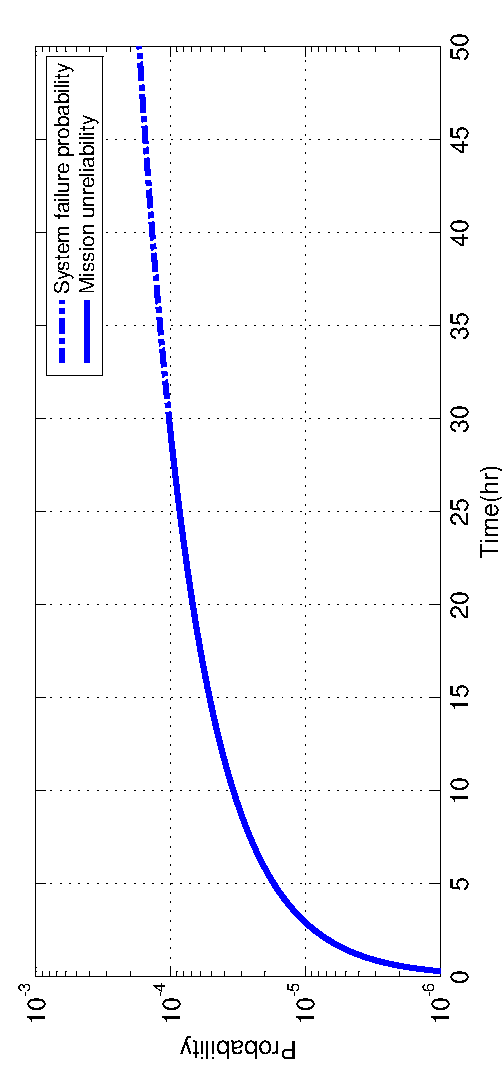
\includegraphics[scale=0.7,angle=-90]{MarkovMissionUnreliability}
  \caption{Mission unreliability of 30 more hrs given that the system survived for $T$=50 hrs[$cov$ =1.0].\label{fig:MarkovMissionUnreliability}} 
\end{figure}

Figure \ref{fig:MarkovMissionUnreliability} plots the probability that the NCCW system fails in the next 30 hrs given that it was reliable for the first 50 hrs. Owing to the memoryless property of the exponential distribution considered for the failure and repair time distributions of the components, it is observed that the mission unreliability of additional 30 hrs is the same as the system failure probability in the initial 30 hrs of system life time.

\begin{figure}[h!] \centering
  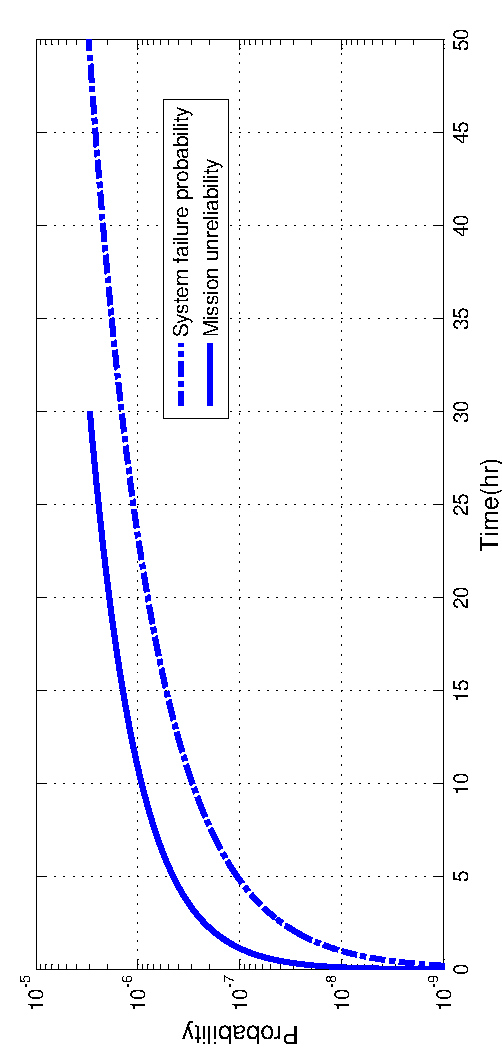
\includegraphics[scale=0.7,angle=-90]{SemiMarkovMissionUnreliability}
  \caption{Mission unreliability of 30 more hours given that the system survived for $T$=50 hrs [$cov$=0.7]. \label{fig:SemiMarkovMissionUnreliability}} 
\end{figure}

Figure \ref{fig:SemiMarkovMissionUnreliability} plots the mission unreliability of the NCCW system assuming Weibull distribution for heat exchanger failure time and exponential distribution for the failure and repair time  of the pump trains. It is observed that the mission unreliability of additional 30 hrs having survived 50 hrs is higher than system failure probability in the initial 30 hrs of system life time. At the end of 80 hrs, the mission unreliability is 2.9647 x $10^{-6}$ and the system failure probability is 3.0380 x $10^{-6}$.


\section*{Truncated distributions}

\begin{align}
g(t)=\frac{f(t)}{F(b)-F(a)} \hspace{0.5in} 0 \leq a \leq t \leq b < \infty
\end{align}
\begin{align}
G(t)=\frac{F(t)-F(a)}{F(b)-F(a)} \hspace{0.5in} 0 \leq a \leq t \leq b < \infty
\end{align}

\begin{figure}[h!] \centering
  \includegraphics[scale=0.7,angle=-90]{TruncatedPdf}
  \caption{Weibull distribution with $\lambda$=0.1 and $\gamma$=3.7 truncated at $a=6, b=10$. \label{fig:TruncatedPdf}} 
\end{figure}

\begin{figure}[h!] \centering
  \includegraphics[scale=0.7,angle=-90]{TruncatedCdf}
  \caption{Weibull distribution with $\lambda$=0.1 and $\gamma$=3.7 truncated at $a=6, b=10$. \label{fig:TruncatedCdf}} 
\end{figure}
  


%% References
%%
%% Following citation commands can be used in the body text:
%%
%%  \citet{key}  ==>>  Jones et al. (1990)
%%  \citep{key}  ==>>  (Jones et al., 1990)
%%
%% Multiple citations as normal:
%% \citep{key1,key2}         ==>> (Jones et al., 1990; Smith, 1989)
%%                            or  (Jones et al., 1990, 1991)
%%                            or  (Jones et al., 1990a,b)
%% \cite{key} is the equivalent of \citet{key} in author-year mode
%%
%% Full author lists may be forced with \citet* or \citep*, e.g.
%%   \citep*{key}            ==>> (Jones, Baker, and Williams, 1990)
%%
%% Optional notes as:
%%   \citep[chap. 2]{key}    ==>> (Jones et al., 1990, chap. 2)
%%   \citep[e.g.,][]{key}    ==>> (e.g., Jones et al., 1990)
%%   \citep[see][pg. 34]{key}==>> (see Jones et al., 1990, pg. 34)
%%  (Note: in standard LaTeX, only one note is allowed, after the ref.
%%   Here, one note is like the standard, two make pre- and post-notes.)
%%
%%   \citealt{key}          ==>> Jones et al. 1990
%%   \citealt*{key}         ==>> Jones, Baker, and Williams 1990
%%   \citealp{key}          ==>> Jones et al., 1990
%%   \citealp*{key}         ==>> Jones, Baker, and Williams, 1990
%%
%% Additional citation possibilities
%%   \citeauthor{key}       ==>> Jones et al.
%%   \citeauthor*{key}      ==>> Jones, Baker, and Williams
%%   \citeyear{key}         ==>> 1990
%%   \citeyearpar{key}      ==>> (1990)
%%   \citetext{priv. comm.} ==>> (priv. comm.)
%%   \citenum{key}          ==>> 11 [non-superscripted]
%% Note: full author lists depends on whether the bib style supports them;
%%       if not, the abbreviated list is printed even when full requested.
%%
%% For names like della Robbia at the start of a sentence, use
%%   \Citet{dRob98}         ==>> Della Robbia (1998)
%%   \Citep{dRob98}         ==>> (Della Robbia, 1998)
%%   \Citeauthor{dRob98}    ==>> Della Robbia


%% References with bibTeX database:
\bibliographystyle{model2-names}

% This specifies the location of the file containing the bibliographic information.  It assumes you're using BibTeX (if not, why not?).
\bibliography{uw-ethesis}
% Tip 5: You can create multiple .bib files to organize your references. 
% Just list them all in the \bibliogaphy command, separated by commas.
%\nocite{*}

%\begin{thebibliography}{14}
%
%
%\end{thebibliography}



\end{document}
